\begin{table}[!t]
\caption{Distinct USWNs and associated sets of \unravelled traces from a single Sepsis Cases Event Log \cite{mannhardt_2016}. $\varepsilon$ represents the machine epsilon \ifdefined\WWITHN and $n=20$ \fi.}\label{tab:dataset}
\centering
 \begin{adjustbox}{max width=\textwidth}
	\begin{tabular}{crl||cl|c}
		\toprule
		\textbf{Experiment Conf.} $(\mathcal{U})$ & \textit{Model} & $+$\textit{W. Estimator} & $p_\theta$& $\;\;|\WCal{p_\theta}{n}(P_{\mathcal{U}})|$ \\
		\midrule
		
		\textbf{SM\_CONS\_20} &SplitMiner 2.0  \cite{AugustoCDRP19}       & +\texttt{Constant} &  $\;\;\varepsilon$ & $157$  \\
		
		\textbf{SM\_FORK\_20} & SplitMiner 2.0  \cite{AugustoCDRP19}      & +Fork \cite{spdwe} &  $\;\;\varepsilon$ & $32$  \\
		
		
		\textbf{SM\_PAIR\_20} & SplitMiner 2.0  \cite{AugustoCDRP19}      & +PairScale \cite{spdwe} &  $\;\;\varepsilon$ & $157$ \\

		\textbf{STPETRI\_20} & \multicolumn{2}{c||}{Rogge-Solti \cite{RoggeSoltiAW13}} &  $10^{-5}$ & $1612$ \\
		\bottomrule
	\end{tabular}
\end{adjustbox}
\end{table}
\section{Experimental Results}\label{sec:exp}
\subsection{Dataset}
For our experiments, we took the Sepsis Cases event log \cite{mannhardt_2016} and split the dataset into a training set, containing the ``\textit{happy traces}''  having duration lower than or equal to the average trace duration in the log ($\leq 2.3\cdot 10^{7}$ ms), and a test set, containing the traces with the highest execution times. We used the training set to generate either a USWN, using the approach presented in \cite{RoggeSoltiAW13}, or a BPMN with only exclusive gates using Split Miner 2.0 \cite{AugustoCDRP19} that was then converted into a Petri net \cite{PPNFromLog}. This Petri net was later on converted into a USWN by using a firing weight estimator: we choose the \texttt{Fork} and the \texttt{PairScale} estimators from \cite{spdwe} and we denote as \texttt{Constant} a naive estimator assuming that all the transition enabled in a given marking are equiprobable. %No estimator was used for the USWN generated via ProM, as such engine already estimates the firing weights.
From such USWNs, we generated distinct sets of \unravelled\ traces (of different sizes). The experimental settings are summarized in \tablename~\ref{tab:dataset}. The experiments described in the following sections have the aim of evaluating the benefits of performing the approximate-ranking strategy over the optimal-ranking one.

\begin{figure*}[!t]
\begin{minipage}{.49\textwidth}
	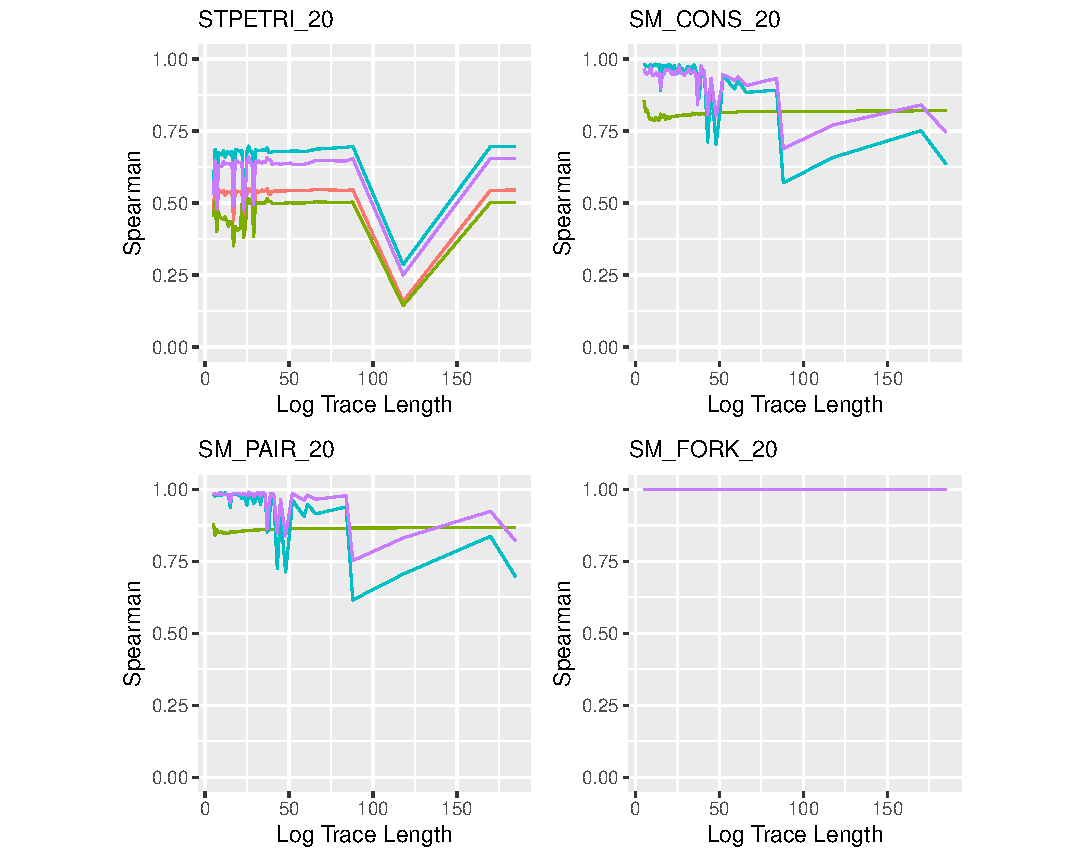
\includegraphics[width=1.1\textwidth]{images/Prec.pdf}
	\caption{Approximation comparison.}\label{fig:app}
\end{minipage}\hfill \begin{minipage}{.49\textwidth}

	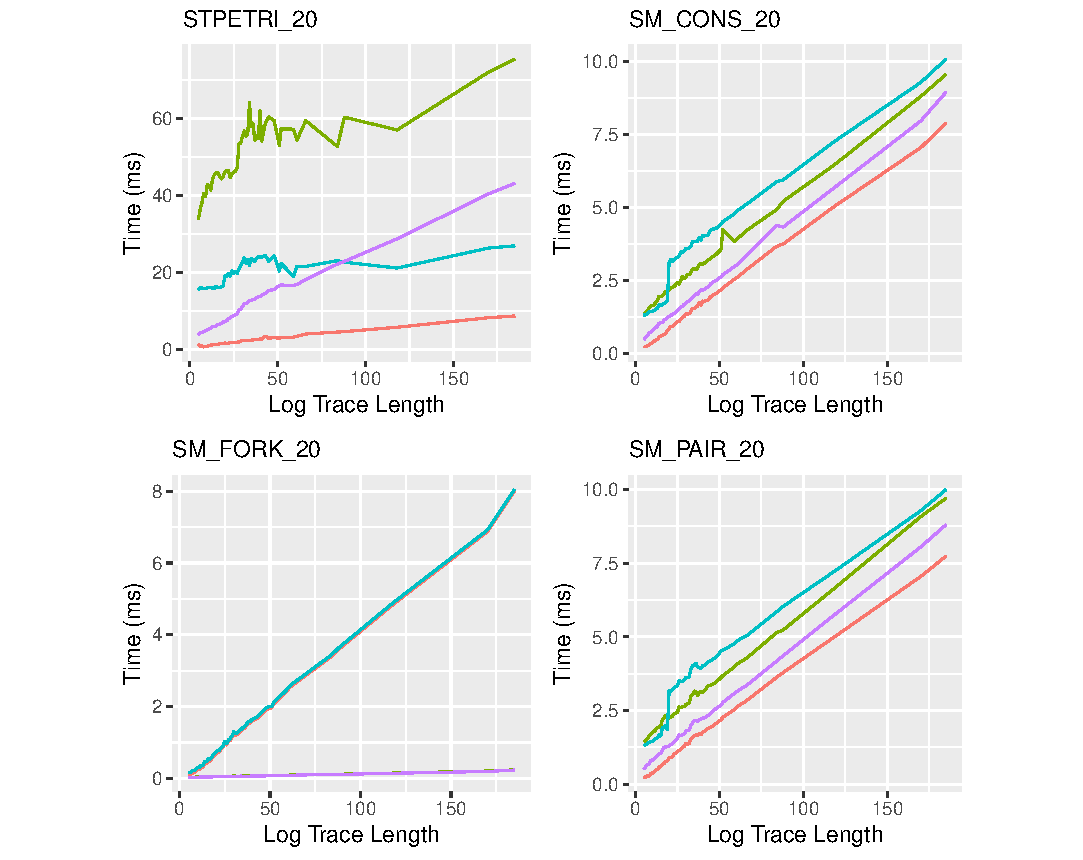
\includegraphics[width=1.1\textwidth]{images/kronos.pdf}
	\caption{$k$NN alignment benchmark.}\label{fig:kronos}
\end{minipage}
\end{figure*}
\subsection{Approximation}\label{subsec:apprp}
In order to assess how well the proposed approximate-ranking strategy approximates the optimal-ranking one, we use the Spearman correlation index \cite{SCI} to express the correlation between the ranking provided by each sub-embedding strategy for $\phi_{\mathcal{P}}$ ($\color{ggplotGreen}\epsilon^1\&\nu^1$, $\color{ggplotRed}\epsilon^2\&\nu^1$, $\color{ggplotPurple}\epsilon^1\&\nu^2$, and $\color{ggplotBlue}\epsilon^2\&\nu^2$) and the optimal ranking. In \figurename~\ref{fig:app}, we show the average Spearman index for traces of different lengths in the test set. We can see from the plots that the sub-embeddings considering only information about the edges (i.e., the ones where the features corresponding to the $\nu$ dimension are set to zero) have in general a higher correlation with the optimal ranking, but their correlation values are less stable with respect to the length of the trace to be aligned. In the case of \textbf{STPETRI\_20}, the correlation is lower than for the other configurations (lower than 0.7 for all sub-embeddings). For \textbf{SM\_PAIR\_20} and \textbf{SM\_CONS\_20}, the correlation index is around 0.8 for $\color{ggplotPurple}\epsilon^1\&\nu^2$ and $\color{ggplotBlue}\epsilon^2\&\nu^2$, and almost 1 for $\color{ggplotGreen}\epsilon^1\&\nu^1$ and $\color{ggplotRed}\epsilon^2\&\nu^1$ but less stable for these sub-embeddings especially for longer traces. In the case of \textbf{SM\_FORK\_20}, the correlation is maximum for all sub-embedding strategies.

%set of \unravelled traces in Table \ref{tab:dataset} and the subset of the Sepsis Cases Event Log that was not used to generate the USWNs. For each of this log trace $\sigma^*$ we added controlled noise (transition addition, deletion, or swap) at either $20\%$ ($\tilde{\sigma}^*$) or $30\%$ ($\tilde{\tilde{{\sigma}}}^*$) of the log trace as for \cite{LeoniM17}. Then, we found the correlation between the ranking $R_\star$ induced by $k_{\phi_{\mathcal{P}}}(\sigma,\sigma^*)$ to the ranking induced by replacing $\sigma^*$ with one of the two noised traces (either a ranking $R_{20}$ induced by $k_{\phi_{\mathcal{P}}}(\sigma,\tilde{\sigma}^*)$ or $R_{30}$ induced by $k_{\phi_{\mathcal{P}}}(\sigma,\tilde{\tilde{\sigma}}^*)$). The correlation $\rho$ between these two rankings ($\rho(R_\star,R_{20})$ and $\rho(R_\star,R_{30})$) is performed via Spearman Correlation Index $\rho$: such index will return near-$1$ on increasing monotonic trend, near-$(-1)$ values on decreasing monotonic trend, and near-$0$ values where the two rankings are almost uncorrelated. Figure \ref{fig:app} shows the outcome of such experiments for all the possible combinations of $\epsilon$ and $\nu$ sub-embeddings for $\phi_{\mathcal{P}}$ while varying the log trace length. We can observe that strategies including traces' frequencies ($\nu^1$) are more stable if compared to strategies where such information is completely ignored ($\nu^2$). Furthermore, such approximation never reaches zero values, while that occurrence might happen for $\nu^2$-based strategies.

\subsection{Efficiency}\label{subsec:efficio}
With reference to the plots in \figurename~\ref{fig:kronos}, we evaluated the efficiency of computing the trace alignment over both optimal-ranking ({\color{ggplotPurple}Purple} and {\color{ggplotGreen}Green}) and approximate-ranking ({\color{ggplotBlue}Blue} and {\color{ggplotRed}Red}) strategies over two different data structures enabling $k$NN queries, i.e., VP-Trees ({\color{ggplotBlue}Blue} and {\color{ggplotPurple}Purple}) and KD-Trees ({\color{ggplotRed}Red} and {\color{ggplotGreen}Green}). We conducted our experiments for $k=20$, and we used the Levenshtein distance as distance function for the optimal-ranking strategy. While the average query time (over traces of the same length) for the optimal-ranking strategy includes the \textit{indexing time} for generating all the vectors of the search space (that has to be constructed from scratch for each query) and the time for the neighborhood search, the approximate-ranking one includes the neighborhood search time and the time needed for the embedding transformation of the trace to be aligned $x$ (in this case, the indexing cost is performed only once before the query time); in particular, in the latter case, in addition to averaging the query time over traces of the same length, we also consider the average embedding time for all the possible embedding strategies introduced in this paper (and also used in the previous section). \figurename~\ref{fig:kronos} plots the result of such experiments: the time required to generate all the alignments needed to compute $\phi_\star(x)$ truly dominates the cost of generating the embedding $\phi_{\mathcal{P}}(x)$ for datasets with a higher number of model traces such as \textbf{STPETRI\_20}, while the cost for $\phi_{\mathcal{P}}(x)$ becomes non-negligible when the model generates a more restricted set of traces and, therefore, we have to compute a lower number of alignments to generate the optimal ranking (like, for example, in the case of \textbf{SM\_FORK\_20}). Finally, we can see that, in general, the computation time increases with the length of the traces to be aligned.
%Last, while the $k$NN alignments over $\phi_{\mathcal{P}}$ always provide the best timing results via KD-Trees, we cannot elect a best data structure $\phi_\star$ that is valid for all datasets and all trace lengths. 